\documentclass[a4paper,12pt]{article}
\usepackage{geometry}
\usepackage{graphicx}
\usepackage{hyperref}
\usepackage{cleveref}
\usepackage{float}

\geometry{left=2.5cm, right=2.5cm, top=2.5cm, bottom=2.5cm}

\title{\textbf{NeuroBrush: Real-Time Artistic Style Transfer System}}
\author{Course: AIT102 - Python and TensorFlow Programming}
\date{\today}

\begin{document}

\maketitle

\section{Group Members}
\begin{table}[h]
    \centering
    \begin{tabular}{|c|c|c|}
        \hline
        \textbf{No.} & \textbf{Name} & \textbf{Student ID} \\
        \hline
        1 & Min Yiduo (Leader) & DSC2409026 \\
        \hline
        2 & Cui Zeyu & DSC2409006 \\
        \hline
        3 & Deng Kailong & DSC2409007 \\
        \hline
        4 & Dong Yanzhe & DSC2409008 \\
        \hline
        5 & Lin Jiacheng & DSC2409018 \\
        \hline
    \end{tabular}
\end{table}

\section{Task Distribution}
\begin{itemize}
    \item \textbf{Min Yiduo}: Model Architecture Design \& Research
    \item \textbf{Deng Kailong}: Dataset Preparation (COCO 2017) \& Preprocessing Pipeline
    \item \textbf{Dong Yanzhe}: Backend Implementation (TensorFlow Training Loop)
    \item \textbf{Cui Zeyu}: Frontend Development (HTML/Flask Web Interface)
    \item \textbf{Lin Jiacheng}: Testing, Optimization \& Assignment Report Writing
\end{itemize}

\section{Model Description}

\subsection{Overview}
Our project aims to implement a Fast Style Transfer system capable of
transforming user-uploaded photos into artistic styles (e.g., Van Gogh, Picasso)
in real-time. Unlike the slow optimization-based method (Gatys et al.
\cite{gatys2015neural}), we will train a feed-forward Image Transformation
Network using the architecture proposed by Johnson et al.
\cite{johnson2016perceptual}

\subsection{Development Phases}

The system consists of two distinct phases: Training Phase and Inference Phase,
as shown in \cref{fig:execution}.

\subsubsection{Training Phase (Development)}
In this phase, we train the Transformation Network to learn a specific style.
\begin{itemize}
    \item \textbf{Dataset}: We use the COCO 2017 Dataset (approx. 80,000 images) to train the network on content recognition.
    \item \textbf{Style Image}: A single artistic image (e.g., \textit{Starry Night}) serves as the target style.
    \item \textbf{Loss Network}: We use a pre-trained VGG-19 network to calculate:
    \begin{itemize}
        \item \emph{Content Loss}: Difference in feature maps between generated image and original content image.
        \item \emph{Style Loss}: Difference in Gram matrices between generated image and style image.
    \end{itemize}
    \item \textbf{Optimizer}: We use Adam optimizer to update the weights of the Transformation Network to minimize the total loss.
\end{itemize}

\subsubsection{Inference Phase (Production)}
Once trained, the VGG-19 Loss Network is discarded. 
\begin{itemize}
    \item \textbf{Input}: User provides a content image (via HTML frontend).
    \item \textbf{Processing}: The trained Transformation Network acts as a filter, processing the image in a single forward pass.
    \item \textbf{Output}: A stylized image is generated in milliseconds.
\end{itemize}

\begin{figure}[H]
    \centering
    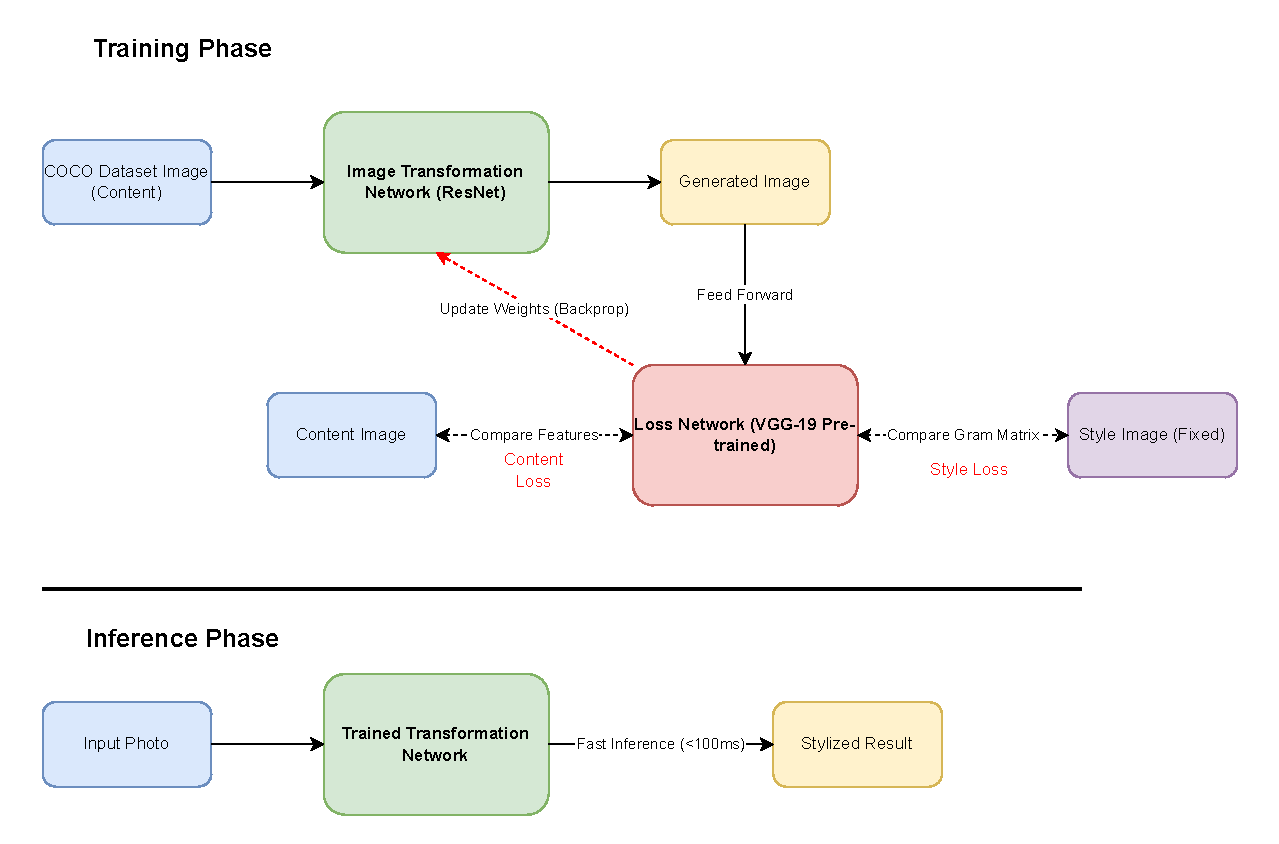
\includegraphics[width=0.9\textwidth]{execution.pdf}
    \caption{Two Phases of Project Development}
    \label{fig:execution}
\end{figure}

\section{System Architecture}
The final application will features a web-based interface, as shown in \cref{fig:architecture}:
\begin{itemize}
    \item \textbf{Frontend}: An HTML5/CSS3 web page allowing users to upload images and select styles.
    \item \textbf{Backend}: A Python Flask server hosting the TensorFlow model.
    \item \textbf{Workflow}: 
    \begin{enumerate}
        \item User uploads image on Web UI.
        \item Image is sent to Python backend.
        \item TensorFlow model performs inference.
        \item Stylized image is returned and displayed on the webpage.
    \end{enumerate}
\end{itemize}

\begin{figure}[H]
    \centering
    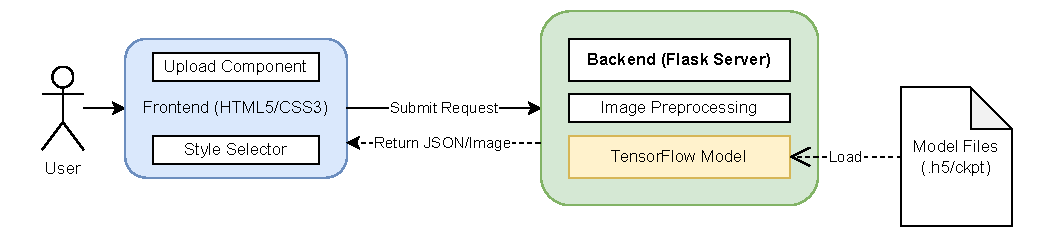
\includegraphics[width=0.9\textwidth]{architecture.pdf}
    \caption{System Architecture}
    \label{fig:architecture}
\end{figure}

\section*{Note on Current Progress (Submission)}
This folder contains the Phase 1 (MVP) of the project. 
\begin{itemize}
    \item We have implemented the complete inference pipeline and image processing utilities.
    \item To demonstrate functionality immediately, the current code utilizes a pre-trained TF-Hub model as a placeholder.
    \item Phase 2 (In Progress): We are currently setting up the training pipeline on the COCO dataset to replace the placeholder with our own custom-trained weights as described above.
    \item Demonstration: \Cref{fig:inputs} shows the input images used for our MVP, and \Cref{fig:result} displays the generated stylized result.
\end{itemize}

\begin{figure}[H]
    \centering
    \begin{minipage}{0.45\textwidth}
        \centering
        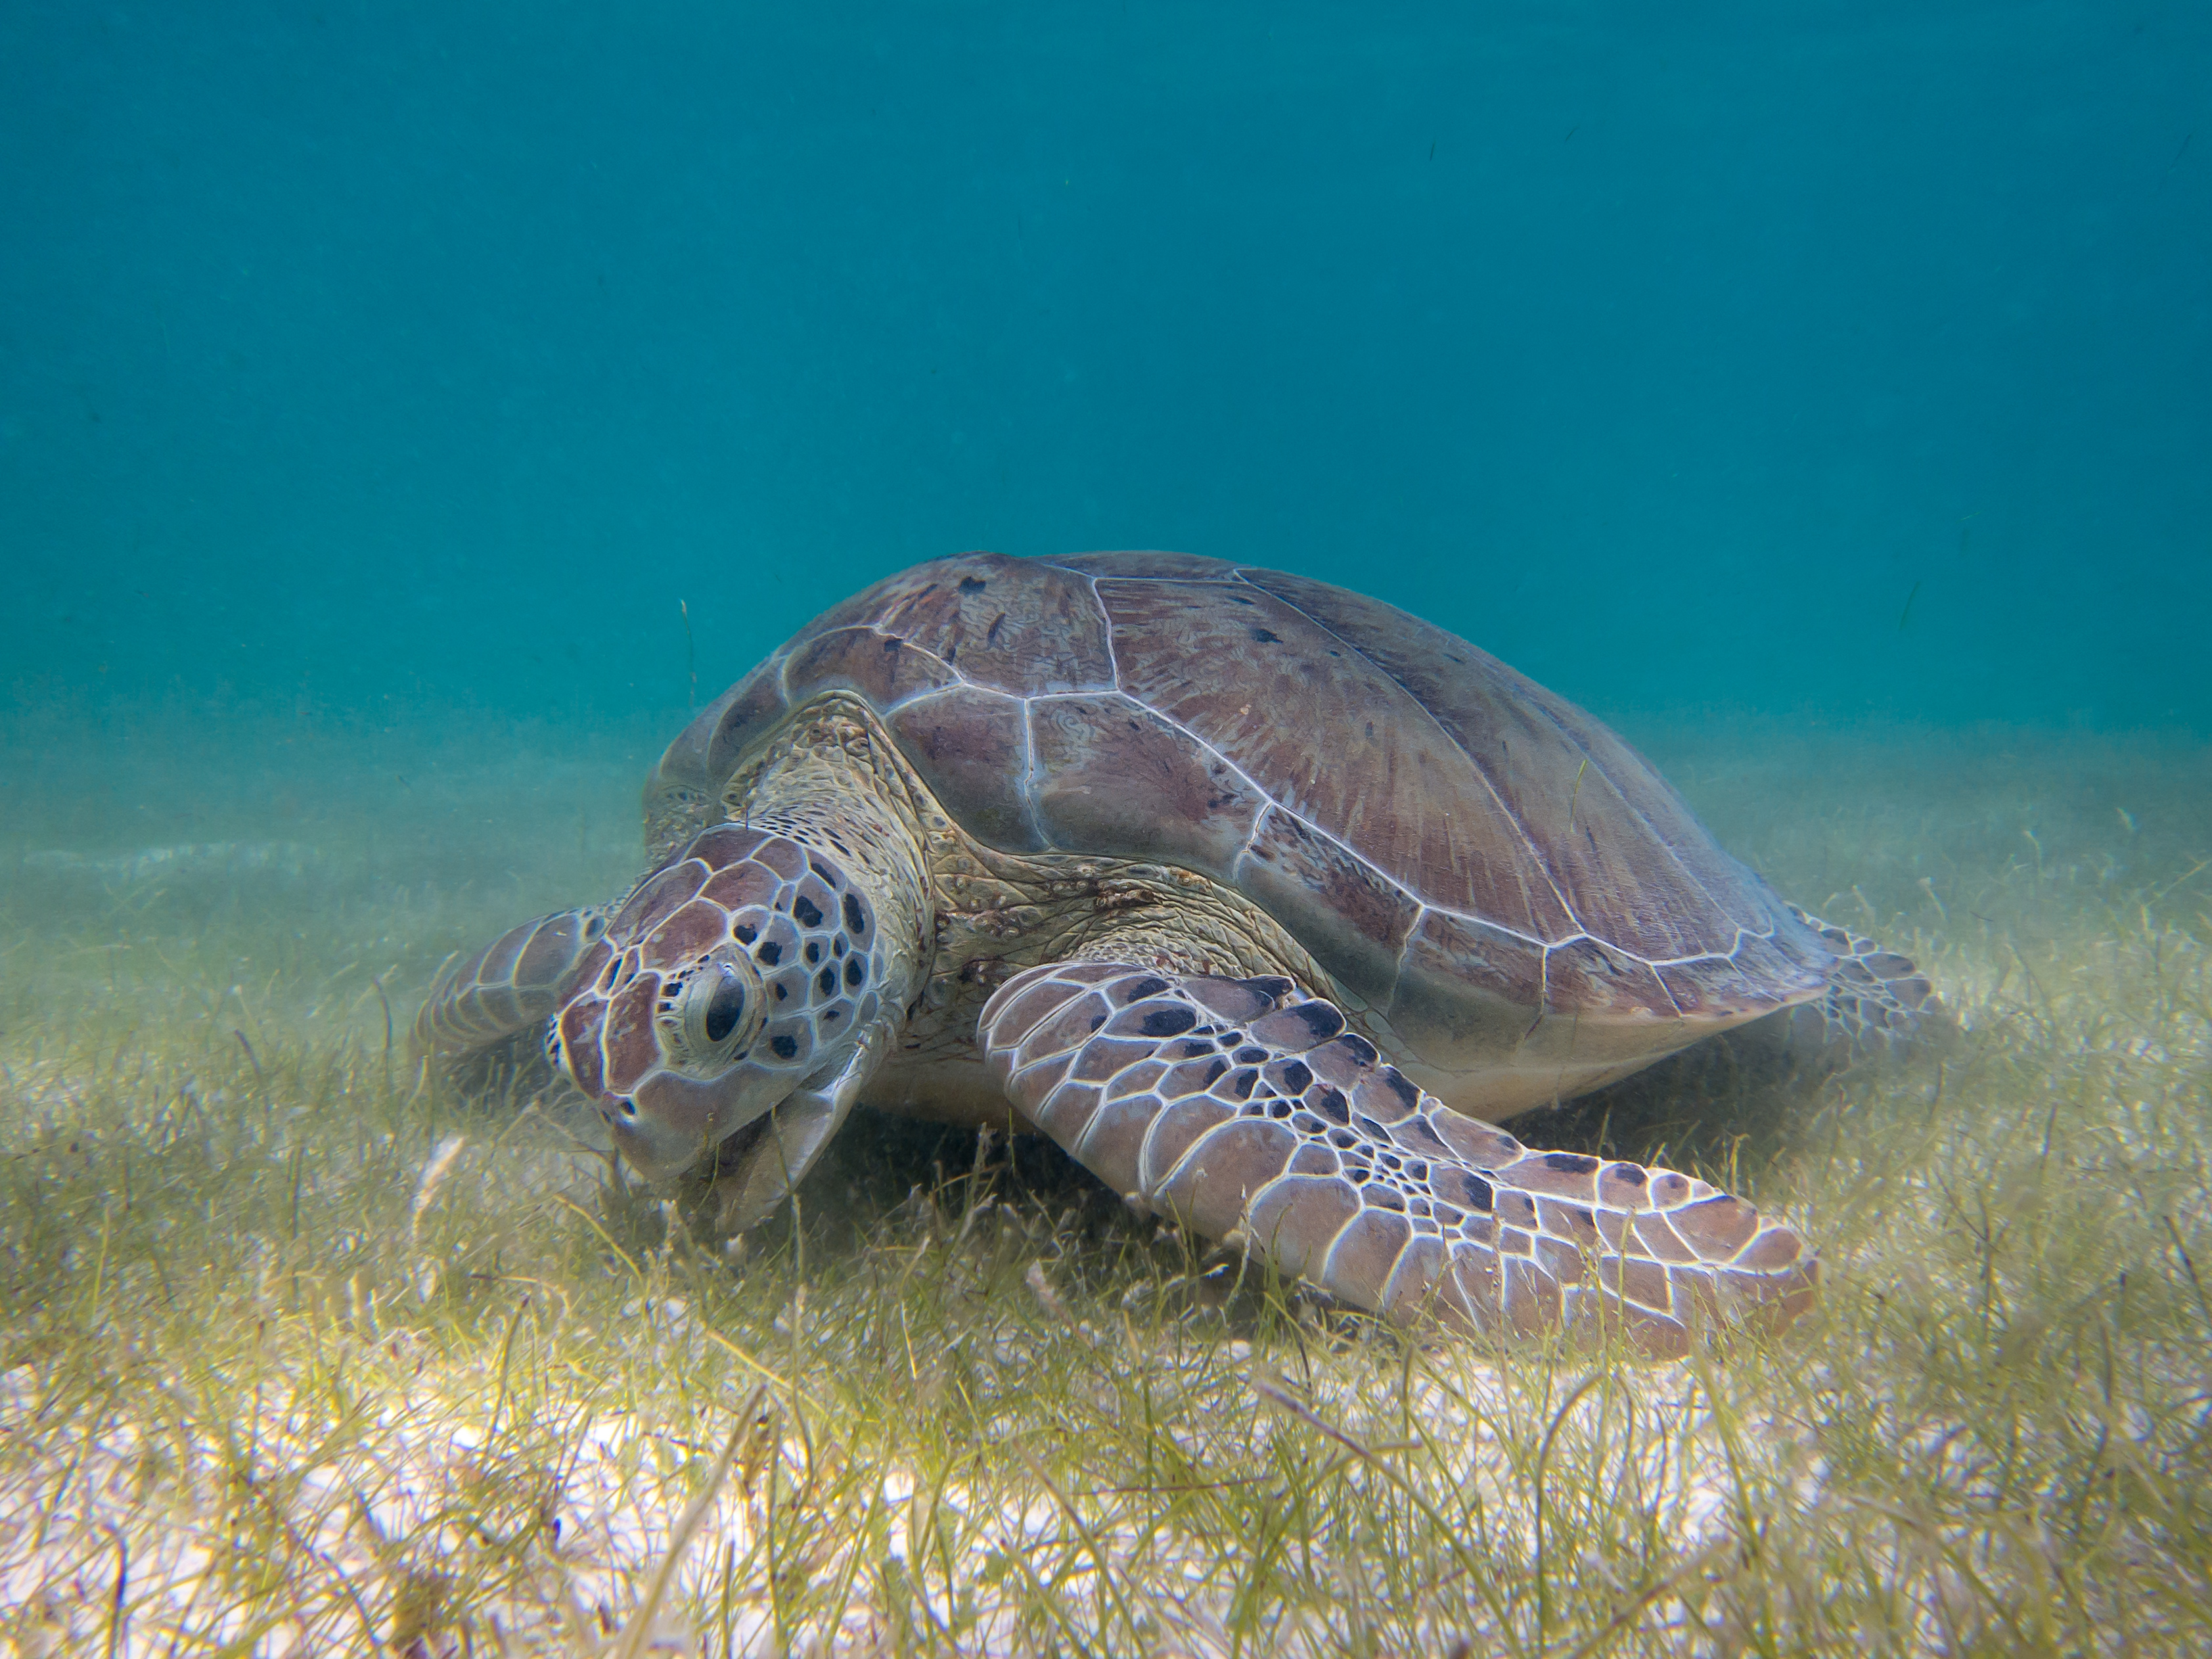
\includegraphics[width=\linewidth]{code/content.jpg}
        \centerline{\textbf{Content Image}}
    \end{minipage}
    \hfill
    \begin{minipage}{0.45\textwidth}
        \centering
        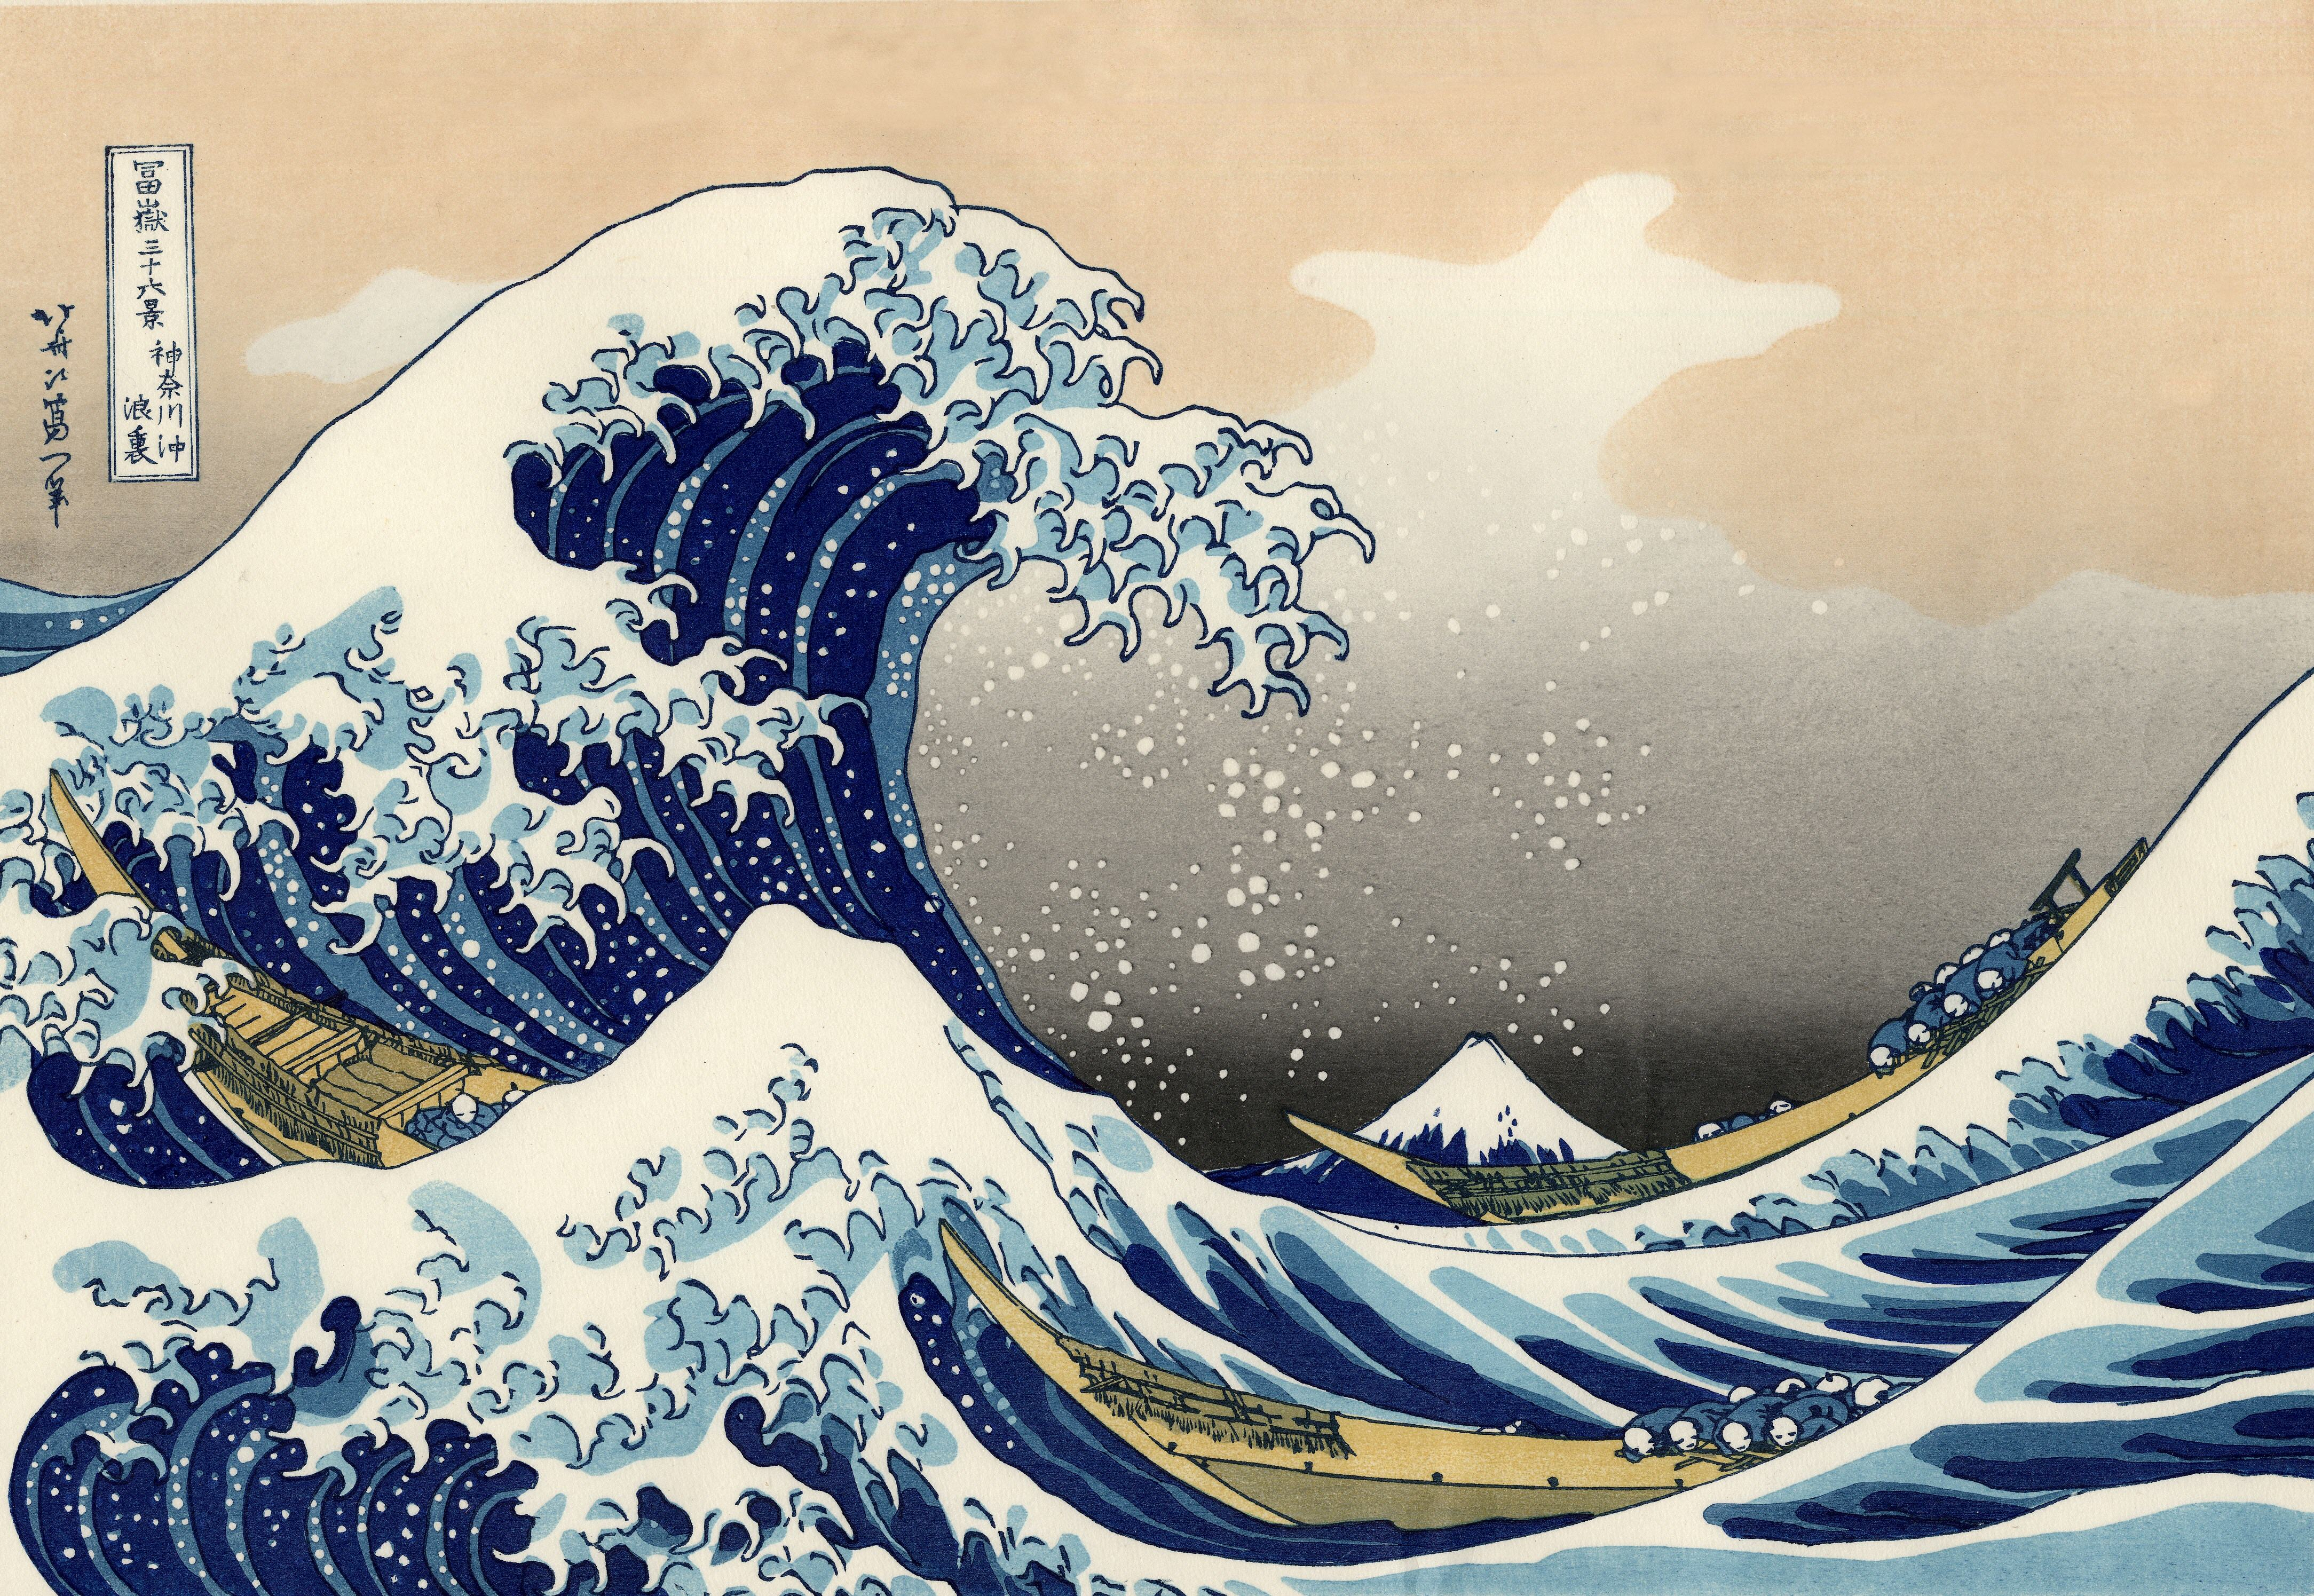
\includegraphics[width=\linewidth]{code/style.jpg}
        \centerline{\textbf{Style Image}}
    \end{minipage}
    \caption{Input Images for Style Transfer}
    \label{fig:inputs}
\end{figure}

\begin{figure}[H]
    \centering
    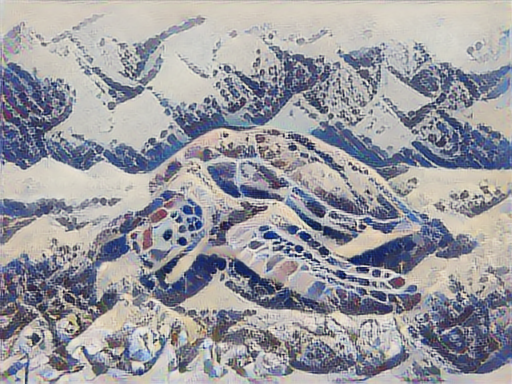
\includegraphics[width=0.6\textwidth]{code/stylized_image.png}
    \caption{Stylized Result (MVP Phase)}
    \label{fig:result}
\end{figure}

\bibliographystyle{plain}
\bibliography{references}

\end{document}
